\documentclass{article}

\usepackage{Sweave}
\begin{document}
\Sconcordance{concordance:Report_Draft.tex:Report_Draft.Rnw:%
1 2 1 1 0 7 1 1 7 1 13 1 2 21 1 1 30 1 13 5 1}


\subsubsection*{Duration of the trials}

The duration of the experiment took on average less in the non-verbal condition (Avg:13.17 min, SD:3.32 min) than in verbal condition (Avg: 17.49 min, SD: 5.80 min)  (Kruskal-Wallis chi-squared = 4.32, df = 1, p-value = 0.03767). The effect of the group is visibile also in the single trial, although the significance o fthe non-parametric test is reached only in the trials 3,5,6,7,8. The is probably due to the manipulationtemptation: the interface results too attractive for the participant and could lead to negative learning outcomes(Do-Lenh, S., Jermann, P., Legge, A., Zufferey, G.,  Dillenbourg, P. (2012). TinkerLamp 2.0: designing and evaluating orchestration technologies for the classroom. In 21st Century Learning for 21st Century Skills (pp. 65-78). Springer Berlin Heidelberg.) 

Between learners and non-learners there is no significant difference.   

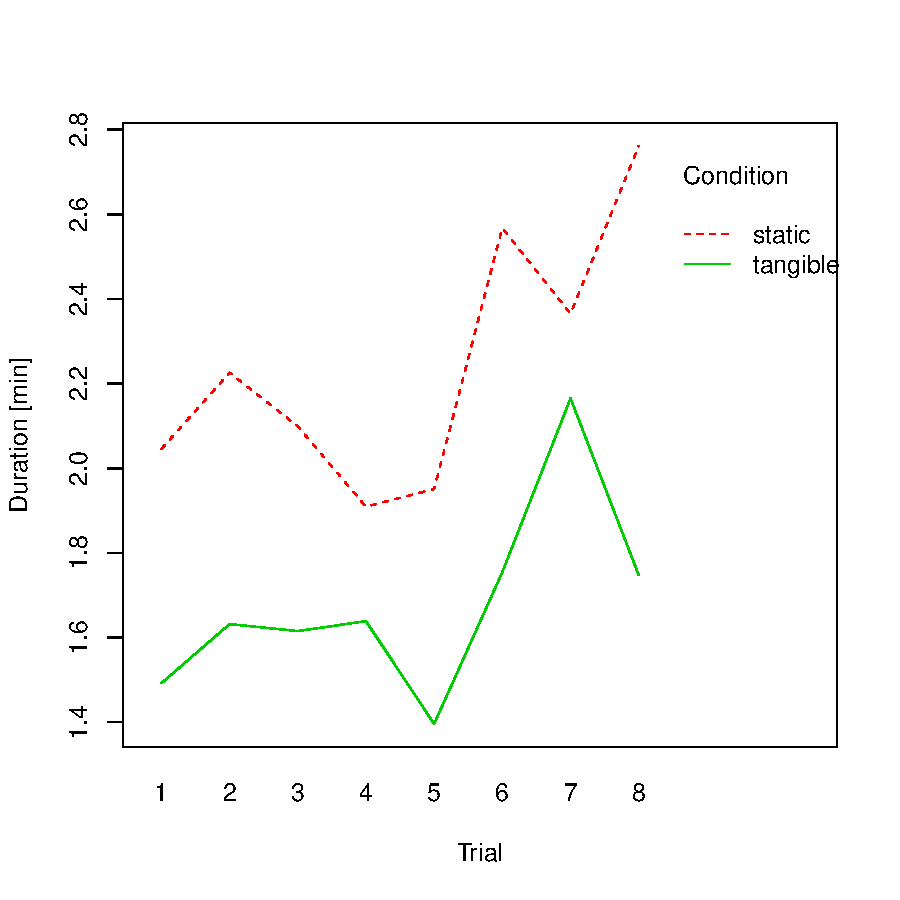
\includegraphics{Report_Draft-002}

In the following tests, we consider the fixation events on areas of interests. The AOI set is made of the joints and beams present in each model. Events that do not interest these areas are discarded. 
Regarding the percentage of fixation time spent on the joints in the overall experiment \footnote{Sum of fixation time on joints divided by total fixation time.}, we found that partipants in verbal condition allocated more time to the joints than the subjects in non-verbal condition (Verbal Avg=40.93\%, SD=4.78\%, Non-Verbal Avg=32.88\%, SD=6.63\%,  Wilcoxon Mann-Whitney Rank Sum Test Z=2.7713 , p=0.004). The effect of the condition is visible in all the trials expect in trial 7. The significance values are reported in the Table.
Learners looked a bit more at the joints, but no significant difference was found.
These results are particularly important for the design of the interface:the current interface shows the effect of the forces on the beams, however, the beams are not relevant for solving the problem in this specific task involving truss analysis. Hence, as sied effect the subjects in non-verbal condition tended to focus on the behaviour of the single beam rather than on its contribution to the equilibrium of one node of the structure.  

\begin{table}[h!]
  \begin{center}
    \begin{tabular}{| l | r |}
    \hline
    Trial & Test Result\\
    1 & Z = 1.8464, p = 0.068\\
    2 & Z = 2.3094, p-value = 0.020\\
    3 & Z = 1.5011, p-value = 0.143\\
    4 & Z = 2.1939, p-value = 0.028\\
    5 & Z = 2.8868, p-value = 0.002\\
    6 & Z = 1.9630, p-value = 0.051\\
    7 & Z = 0.0615, p-value = 0.975\\
    \hline
    \end{tabular}
  \end{center}
\end{table}
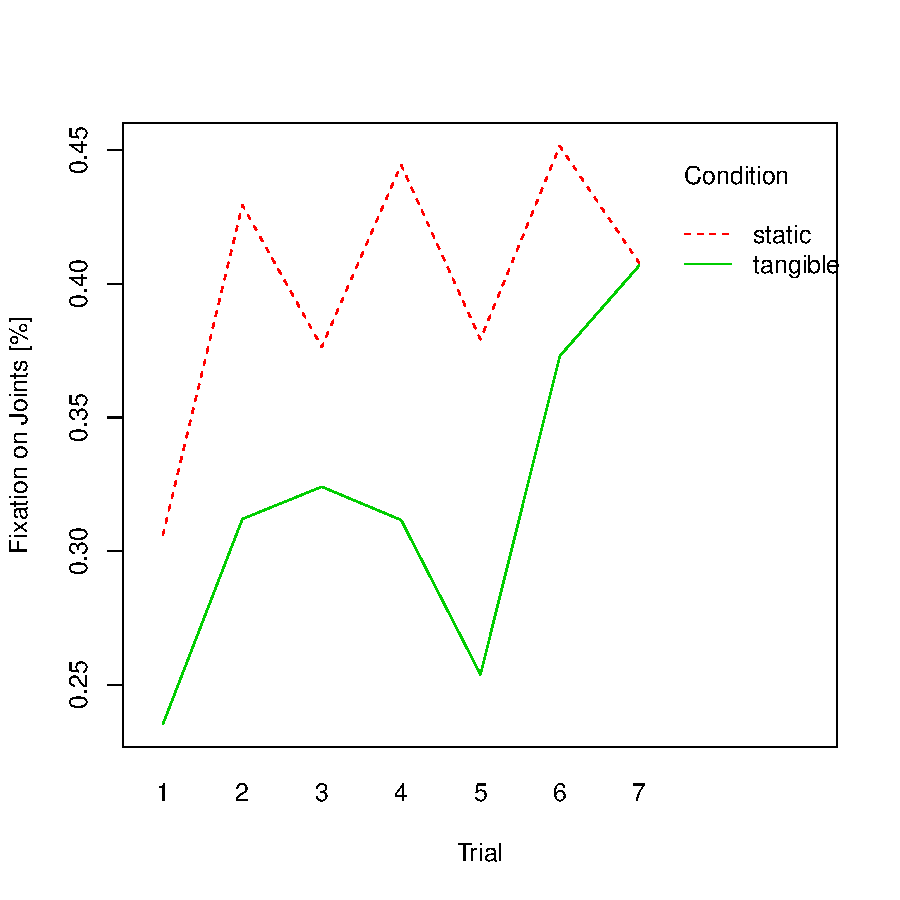
\includegraphics{Report_Draft-003}

This hypothesis is also supported by the results of the average dwell duration on the beams: participant in non-verbal condition showed an increment of 74 ms compared to the ones in verbal condition (linear mixed model, Chisq(1)=4.8746,p=0.02725) and longer dwell on those areas compared to the ones on the beams (+54ms, linear mixed model, Chisq(1)=18.523,p<0.000) 



\end{document}
